\documentclass[aspectratio=169,12pt]{beamer}
\usetheme{Madrid}
\usecolortheme{dolphin}
\usefonttheme{professionalfonts}
\setbeamertemplate{navigation symbols}{}
\setbeamertemplate{footline}{}

\usepackage[T1]{fontenc}
\usepackage[utf8]{inputenc}
\usepackage{graphicx}
\usepackage{amsmath,amssymb}
\usepackage{hyperref}
\usepackage{siunitx}
\usepackage{physics}
\usepackage{braket}

\graphicspath{{../../figures/}}

\title[Module B2]{Module B2: Qiskit -- module \texttt{circuit}}
\author{JAMOTTE Maxime, SCHOONEN Cédric}
\institute{Digital Learning Hub}
\date{}

\begin{document}

\begin{frame}
  \titlepage
\end{frame}

\begin{frame}{Objectifs du module B2}
  \begin{itemize}
    \item Construction de circuits avec \texttt{QuantumCircuit}\\~\\
    \item Matrices derrière les portes logiques\\~\\
    \item Construction d'une paire de Bell\\~\\
    \item JN = Jupyter Notebook
  \end{itemize}
\end{frame}

% ============================================================
\section{Construction de circuits}
% ============================================================

\begin{frame}{Circuits quantiques à un qubit (voir JN)}
  \begin{itemize}
    \item Un circuit logique est un ensemble d'opérations logiques opérées sur un état d'entrée.\\~\\
    \item En Qiskit: créer un circuit avec \texttt{QuantumCircuit(n)}.\\~\\
    \item Ajouter des portes: \texttt{qc.h(0)}, \texttt{qc.x(0)}, \texttt{qc.z(0)}.\\~\\
    \item Visualiser: \texttt{qc.draw('mpl')}.
  \end{itemize}
\end{frame}

\begin{frame}{Circuits à un qubit: exemples}
  \begin{columns}[T,onlytextwidth]
    \column{0.48\textwidth}
    \centering
    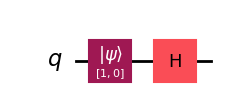
\includegraphics[width=0.8\linewidth]{gate_hadamard.png}
    \\[-0.3em]\footnotesize Circuit: $H$
    
    \vspace{1em}
    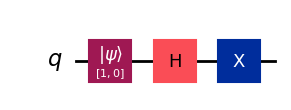
\includegraphics[width=0.8\linewidth]{gate_h_then_x.png}
    \\[-0.3em]\footnotesize Circuit: $H$ puis $X$
    \column{0.48\textwidth}
    \centering
    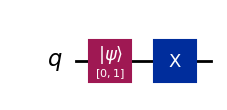
\includegraphics[width=0.8\linewidth]{gate_x.png}
    \\[-0.3em]\footnotesize Circuit: $X$
    
    \vspace{1em}
    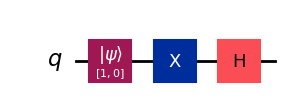
\includegraphics[width=0.8\linewidth]{gate_x_then_h.png}
    \\[-0.3em]\footnotesize Circuit: $X$ puis $H$
  \end{columns}
\end{frame}

% ============================================================
\section{Matrices derrière les portes logiques}
% ============================================================

\begin{frame}{Matrices derrière les portes (voir JN)}
  \begin{itemize}
    \item Chaque porte quantique correspond à une matrice unitaire.\\~\\
    \item On peut extraire la matrice d'un circuit avec \texttt{Operator(qc).data}.\\~\\
    \item Vérification: le produit matrice-vecteur donne le même résultat que \texttt{Statevector.from\_instruction}.
  \end{itemize}

  \vspace{1em}
  \[
    H = \frac{1}{\sqrt{2}}
    \begin{pmatrix} 1 & 1 \\ 1 & -1 \end{pmatrix},
    \qquad
    X = \begin{pmatrix} 0 & 1 \\ 1 & 0 \end{pmatrix},
    \qquad
    Z = \begin{pmatrix} 1 & 0 \\ 0 & -1 \end{pmatrix}
  \]
\end{frame}

% ============================================================
\section{Construction d'une paire de Bell}
% ============================================================

\begin{frame}{Circuit pour une paire de Bell (voir JN)}
  \begin{itemize}[<+->]
    \item On construit un circuit à 2 qubits.\\~\\
    \item On applique $H$ sur le premier qubit: \texttt{qc.h(0)}.\\~\\
    \item On applique CNOT: \texttt{qc.cx(0, 1)}.\\~\\
    \item L'état final est $\ket{\Phi_+} = \frac{1}{\sqrt{2}}(\ket{00}+\ket{11})$.
  \end{itemize}
  \begin{center}
    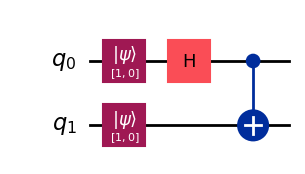
\includegraphics[width=0.4\textwidth]{bell_pair.png}
  \end{center}
\end{frame}

\begin{frame}{Mesure de la paire de Bell (voir JN)}
  \begin{itemize}
    \item Ajout de bits classiques et mesure: \texttt{qc.measure\_all()}.\\~\\
    \item Résultats: uniquement $\ket{00}$ et $\ket{11}$, chacun avec probabilité $\approx 0.5$.
  \end{itemize}
  \begin{center}
    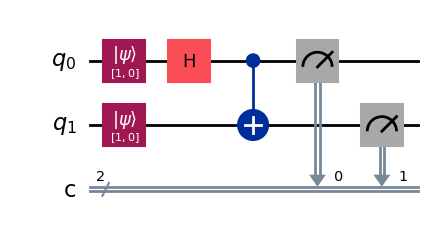
\includegraphics[width=0.45\textwidth]{bell_pair_mesures.png}\hfill
    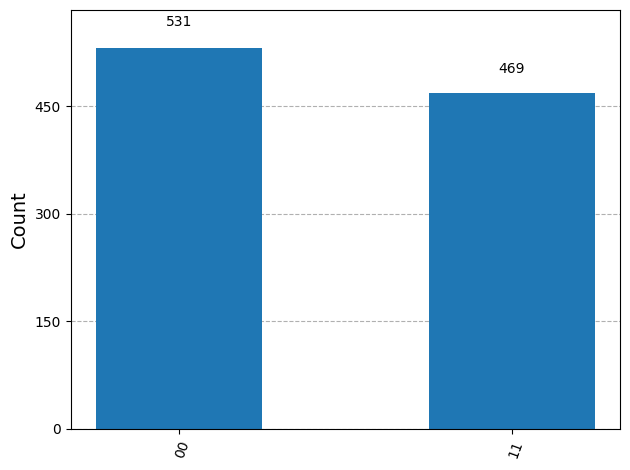
\includegraphics[width=0.45\textwidth]{bell_hist.png}
  \end{center}
\end{frame}

\begin{frame}{Fin du module B2}
  \centering
  \vfill
  Passons à l'exécution sur un vrai QPU!
  \vfill
\end{frame}

\end{document}
